\chapter{Processore MIPS}
Il \textbf{processore MIPS} (Microprocessor without Interlocked Pipeline Stages) è un'architettura RISC progettata per essere semplice ed efficiente. Usa un set ridotto di istruzioni, tutte della stessa lunghezza (32 bit), e adotta una pipeline a 5 stadi per eseguire le istruzioni in modo parallelo.

\section{Architettura MIPS} \label{sec:mips}
L'\textbf{architettura del MIPS} è un'architettura di tipo RISC che consiste di una \textit{integer processing unit} (la CPU) e un insieme di \textit{coprocessori} (fino a 4) [\ref{fig:mips_arc}]. Lo standard richiede obbligatoriamente la presenza del coprocessore 0, mentre per gli altri viene lasciata libertà di decisione a chi lo implementa.
\begin{figure}[!h]
    \centering
    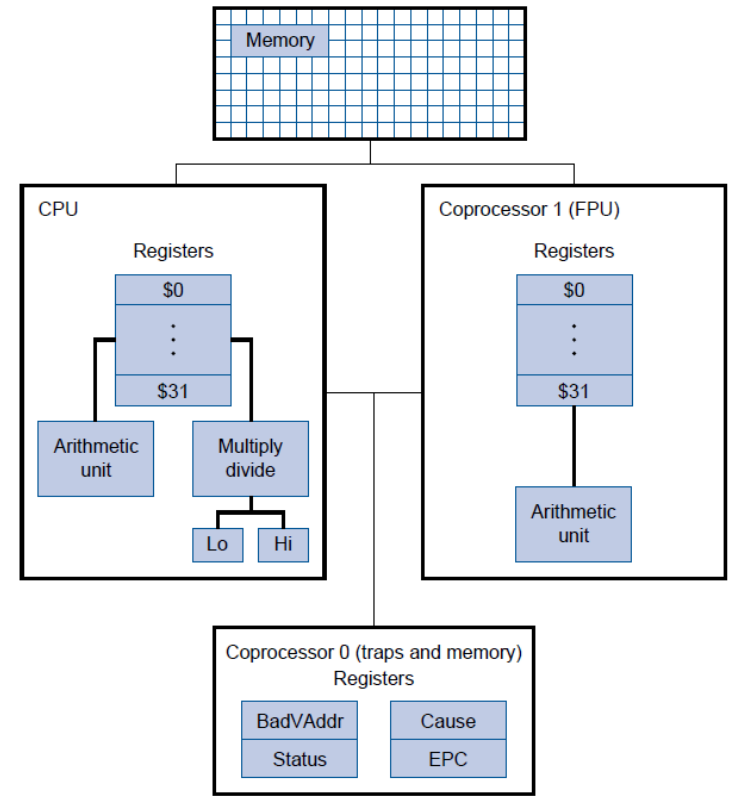
\includegraphics[width=0.45\linewidth]{img/mips.png}
    \caption{Architettura del MIPS.}
    \label{fig:mips_arc}
\end{figure}
Nello specifico, la CPU dispone di 32 registri general purpose a 32 bit per operazioni su interi. Il coprocessore 0 contiene le informazioni necessarie alla gestione delle eccezioni e interruzioni, oltre che lo Status Register (SR). Mentre il coprocessore 1 è la floating point unit, e consiste di 32 registri general purpose a 32 bit per operazioni in virgola mobile. Il processore ha due modalità di funzionamento, dette \textit{user} e \textit{kernel} mode. I task utente non possono in alcun modo accedere alle risorse di memoria dedicate ai task kernel, incluse le strutture dati del sistema operativo e i dispositivi di I/O. Inoltre, i task utente non possono in alcun modo modificare il funzionamento della macchina, in quanto non possono accedere al coprocessore 0.
\\
\\
Notiamo dall'architettura come le operazioni di moltiplicazione e divisione siano gestite da una componente hardware separata e che lavora su due registri speciali (HI e LO). Il motivo è che queste operazioni richiedono molti cicli di clock, e interromperle potrebbe essere troppo oneroso.
\\
\\
Il MIPS ha un'architettura della memoria totalmente diversa rispetto a quella presentata nel classico modello di Von Neumann, ispirandosi al modello Harvard che prevede due memorie separate per dati e istruzioni (anche se queste condividono lo stesso spazio fisico) [\ref{fig:mem-mips}]. Inoltre, all'interno della CPU viene posta una piccola memoria veloce che contiene una serie di registri generali utilizzabili durante le istruzioni, nota come \textit{Register File}. Tale memoria ha due porte di lettura e una di scrittura, per cui può leggere da due registri contemporaneamente (ad esempio, dove sono gli operandi) e scriverne uno solo alla volta (ad esempio, per salvare il risultato).
\begin{figure}[!h]
	\centering
	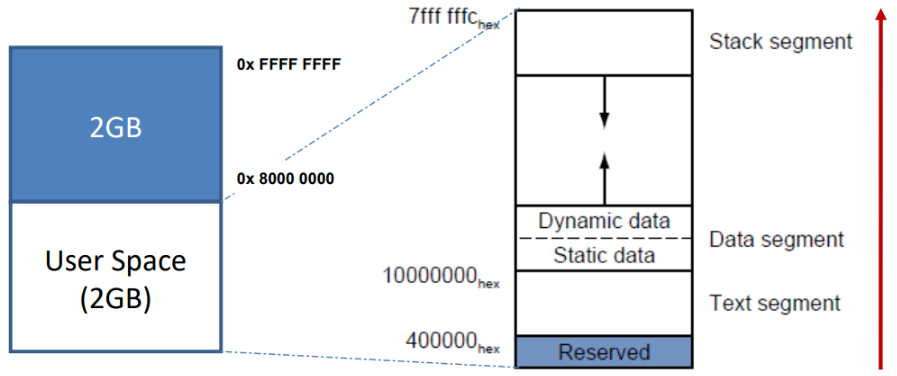
\includegraphics[width=0.5\linewidth]{img/mem-mips}
	\caption{Organizzazione della memoria nel MIPS.}
	\label{fig:mem-mips}
\end{figure}

\section{Gestione delle interruzioni}
Per quanto riguarda la \textbf{gestione delle interruzioni}, questa avviene completamente in software, grazie anche all'uso dl coprocessore 0 che ha il compito di memorizzare tutte le informazioni necessarie. I due registri utilizzati sono Status, che contiene l'interrupt mask, e Cause, che invece contiene il tipo di interruzione e le interruzioni pendenti. Infine, il registro EPC contiene l'indirizzo che ha causato l'eccezione, in modo da poter permettere di ritornare dopo aver eseguito la ISR. Diversamente da quanto accade nel Motorola 68000, è presente un unico Interrupt Handler richiamato da qualsiasi tipo di interruzione. Tale routine risulterà particolarmente complessa, in quanto deve decidere cosa fare in base al tipo di interrupt generata e ai bit presenti nel registro di stato (un vero e proprio switch-case). Più precisamente:
\begin{enumerate}
	\item In seguito a un eccezione o un'interruzione, il processore MIPS salta all'indirizzo che contiene l'exception handler.
	\item Il codice contenuto a tale indirizzo esamina la causa dell'eccezione e invoca il sistema operativo, il quale effettua le dovute operazioni (sospensione di un processo, caricamento di una pagina, lettura o scrittura su I/O).
	\item Dopo aver gestito l'eccezione/interruzione, l'handler ritorna all'istruzione contenuta in EPC oppure a quella immediatamente seguente.
\end{enumerate}
Una tale gestione semplifica notevolmente l'hardware, lasciando una gestione flessibile al sistema operativo.

\section{Pipeline nel MIPS}
Le fasi fondamentali che caratterizzano la pipe del MIPS differiscono leggermente da quelle nel caso generale descritto nell'apposito capitolo [\ref{par:pipe}]. Queste sono:
\begin{itemize}
    \item \textbf{Instruction Memory (IM)}: Si preleva l'istruzione dalla memoria delle istruzioni e si incrementa il Program Counter.
    \item \textbf{Register File (Reg)}: L'istruzione viene decodificata, si prelevano degli operandi dai registri generali presenti nel register file e si preparano i segnali di controllo per la fase di esecuzione.
    \item \textbf{Execute (EX)}: Vengono eseguite le operazioni logico-aritmetiche pilotate dai segnali della fase precedente, oppure calcolato l'indirizzo di memoria per eventuali operazioni di \textit{load} e \textit{store}. In caso di istruzione di salto, si calcola l'indirizzo a cui saltare.
    \item \textbf{Data Memory (DM)}: Avviene la lettura o scrittura dalla memoria dati. Le istruzioni ALU semplici saltano questa fase.
    \item \textbf{Register File (Reg)}: Il risultato dell’ALU o il dato letto dalla memoria viene scritto nel registro di destinazione.
\end{itemize}
\begin{figure}[!h]
    \centering
    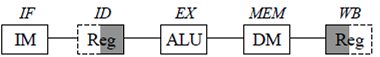
\includegraphics[width=0.5\linewidth]{img/MIPS_clock_split.png}
    \caption{Divisione temporale delle fasi della pipeline nel MIPS.}
    \label{fig:mips-pipe}
\end{figure}

\subsection{Ipotesi di funzionamento}
Analizziamo come l'architettura del MIPS garantisca il soddisfacimento delle ipotesi fondamentali della pipeline.
\\
\\
Come per tutte le architettura pipelined, anche il MIPS richiede che tra le varie fasi vi siano dei registri che conservino lo stato dell'operazione.
Il MIPS, pertanto, presenta vari casi di conflitto che richiedono delle \textbf{ipotesi} sul sistema stesso. Tali ipotesi sono:
\begin{itemize}
    \item \textbf{Velocità della memoria}: La memoria che sarà utilizzata dal MIPS sarà acceduta molto frequentemente (precisamente 5 volte in più rispetto al caso senza pipe).
    \item \textbf{Concorrenze sulla memoria}: Presenza di due memorie, una per le istruzioni ed una per i dati. Tali memorie vengono previste per evitare la concorrenza tra la fase di fetch (prelievo dell'istruzione dalla memoria) e la fase di MEM (lettura o scrittura dalla memoria). 
    \item \textbf{Concorrenza sui registri}: Potenzialmente sul register file possono verificarsi dei conflitti, in particolare quando contemporaneamente un'istruzione vi accede in lettura e una in scrittura. Per risolvere il conflitto, le operazioni di lettura e scrittura vengono effettuate in due intervalli separati dello stesso ciclo di clock, e in particolare la fase di decode (lettura) opera nella seconda parte del ciclo di clock, mentre la fase di write back (scrittura) opera nella prima parte, come riportato in figura \ref{fig:mips-pipe}.
\end{itemize}

\subsection{Istruction Memory}
La \textbf{fase di Istruction Memory} è caratterizzata da 2 operazioni, quella di prelievo dell'indirizzo e quella di incremento del PC. L'istruzione viene letta dalla Instruction Memory (indirizzata dal PC) e posta nel registro di comunicazione tra le fasi di IM e Reg. Dopodiché, il PC viene incrementato e copiato nel registro di comunicazione, perché potrebbe, nel caso di istruzioni di salto, servire a fasi successive.
Pertanto la sua parte architetturale è formata dalle componenti:
\begin{itemize}
    \item \textbf{ADD}: Per favorire l'incremento del PC (che avviene molto frequentemente), l'operazione viene effettuata da un circuito dedicato, in modo da calcolare il prossimo indirizzo del PC senza interferire con altre operazioni dell'ALU.
    \item \textbf{MUX}: Sceglie se considerare l'indirizzo di memoria successivo del PC o un registro di memoria dettato dalla fase di MEM (caso di istruzioni di salto).
    \item \textbf{PC}: Registro Program Counter.
    \item \textbf{Istruction Memory}: Prelievo dell'istruzione da eseguire dalla memoria.
\end{itemize}

\subsection{Register File (ID)}
Nella \textbf{fase di Register File}, il MIPS va a decodificare ed interpretare il comando. In particolare, vengono letti gli eventuali registri sorgente (nel caso di indirizzamento register o immediato) e memorizzati nel registro di comunicazione tra Reg e ALU. Nel caso di istruzioni con indirizzamento immediato, i 16 bit del valore vengono prima convertiti in un valore a 32 bit estendendo il segno. Inoltre, il valore del PC precedentemente passato dalla fase di IM viene propagato insieme ad altre informazioni al registro di comunicazione successivo. Osserviamo che il registro destinazione in cui memorizzare il dato nella fase Reg finale deve essere propagato lungo tutta la pipeline.
Le parti che compongono l'architettura di questa fase sono:
\begin{itemize}
    \item \textbf{Registri}: Registri interni del processore che possono essere pilotati sia in lettura che in scrittura tramite dei segnali esterni.
    \item \textbf{Estensione del segno}: Blocco di estensione con segno dei possibili valori immediati contenuti nell'istruzione.
\end{itemize}
Il blocco estensione del segno è fondamentale perché l'architettura MIPS utilizza istruzioni di lunghezza fissa di 32 bit per semplificare il design del processore e migliorare la velocità di decodifica, e dunque la codifica dei valori acceduti con indirizzamento immediato è fissata a 16 bit. L'estensione a 32 bit è necessaria perché garantisce che il valore immediato possa essere direttamente utilizzato per le operazioni aritmetiche o logiche con i registri (che sono anch'essi a 32 bit).

\subsection{ALU}
Nella \textbf{fase ALU} viene eseguita effettivamente l'istruzione. In particolare, vengono prelevati i dati e i bit di controllo dal registro Reg/ALU e vengono effettuate le operazioni logico-aritmetiche dalla ALU. I risultati vengono memorizzati nel registro di comunicazione tra ALU e DM. In caso di istruzioni di salto, viene presa la decisione di saltare o meno, e viene calcolato il nuovo valore di PC, che viene inserito sempre nel registro di comunicazione ALU e DM. In caso di istruzioni \textit{load} o \textit{store}, viene calcolato l'indirizzo dell'operando in memoria e posto nel solito registro intermedio delle fasi. 
La parte architetturale è composta da vari componenti:
\begin{itemize}
    \item \textbf{ADD}: Strumento che viene utilizzato per calcolare un eventuale offset rispetto ad un valore, e viene utilizzato per calcolare il nuovo valore del PC in caso di salti condizionati o incondizionati.
    \item \textbf{LEFT SHIFT 2}: Moltiplica per 4 il valore per cui voglio saltare (in modo da saltare a 4 indirizzi più avanti).
    \item \textbf{ALU}: Strumento di calcolo aritmetico-logico.
    \item \textbf{MUX}: Seleziona o il dato immediato o un secondo dato proveniente da un registro, proveniente dalla fase precedente.
\end{itemize}

\subsection{Data Memory}
Nella \textbf{fase di Data Memory} avviene l'accesso alla memoria dati, secondo l'indirizzo comunicato dalla fase precedente nel registro ALU/DM. In caso di istruzione di \textit{load}, il dato viene letto e propagato nel registro DM/Reg. La sua architettura è composta principalmente dal singolo elemento di accesso alla memoria dati.

\subsection{Register File (WB)}
Nella seconda \textbf{fase di Register File} si verifica cosa bisogna scrivere all'interno dei registri interni. Il componente che meglio indica il suo funzionamento è il multiplexer finale, che serve per specificare se il dato da caricare all'interno dei registri sia il risultato dell'ALU o qualche valore proveniente dalla memoria dati. 

\section{Gestione dei salti}
Il MIPS adotta una strategia di \textbf{gestione dei salti} molto diversa da quella discussa nel caso generale. Infatti, subito dopo un'istruzione di salto, c'è una \textit{branch delay slot}: l'istruzione successiva viene sempre eseguita, indipendentemente dal risultato del salto. Lo scopo è mantenere la pipeline piena e attiva mentre si valuta il salto. La decisione se saltare o meno avviene nella fase ID, ma nel frattempo (come sappiamo dal comportamento generale) la pipeline ha già precaricato l'istruzione successiva, detta \textit{delay slot}. A quel punto possono verificarsi due situazioni:
\begin{enumerate}
	\item Se il salto non viene effettuato, si continua semplicemente con l'esecuzione della successiva istruzione.
	\item Se il salto viene effettuato, si esegue sempre prima la delay slot e poi si passa all'istruzione situata all'indirizzo del salto.
\end{enumerate}
Per quanto detto, il MIPS non usa predizione dei salti, ma fa sempre l'assunzione che il salto non sarà preso (predict-not-taken) e in caso contrario esegue comunque le istruzioni che non sarebbero dovute essere eseguite (la delay slot) per evitare di sprecare cicli di clock. Questo presuppone che sia il programmatore a fare attenzione a non piazzare istruzioni "sensibili" dopo salti.
\\
\\
\MakeUppercase{è} assolutamente importante, a causa della strategia di gestione dei salti adottata, inserire sempre un'istruzione utile dopo un salto, altrimenti la branch delay slot rimarrebbe indefinita. Per poter realizzare questa accortezza, si inserisce un'istruzione NOP (no operation) dopo il salto nel caso in cui non ci siano istruzioni successive da eseguire.


